\chapter{Multilevel Security}

	A military database systems, which can hold information at a number of different levels 
	of classification (Confidential, Secret, Top Secret, . . .), have to ensure that data can 
	only be read by a principal whose level is at least as high as the data’s classification. 
	The policies they implement are known as {\bf multilevel secure} or alternatively as 
	{\bf mandatory access control} or {\bf MAC}.

	\section{What Is a Security Policy Model?}

		Where a top-down approach to security engineering is possible, it will 
		typically take the form of {\bf threat model — security policy — security mechanisms}. 
		The critical, and often neglected, part of this process is the security policy.
		By a security policy, we mean a document that expresses clearly and
		concisely what the protection mechanisms are to achieve. It is driven by our
		understanding of threats, and in turn drives our system design. It will often
		take the form of statements about which users may access which data. 

		Many organizations use the phrase ‘security policy’ to mean a collection of
		vapid statements. Here is an example:

		\begin{enumerate}
			\item This policy is approved by Management.
			\item All staff shall obey this security policy.
			\item Data shall be available only to those with a ‘need-to-know’.
			\item All breaches of this policy shall be reported at once to Security.
		\end{enumerate}

		This is a typical corporate information security policy.
		This sort of waffle is very common but is useless to the security engineer.

		{\bf A security policy model} is a succinct statement of the protection properties
		which a system, or generic type of system, must have. Its key points can
		typically be written down in a page or less. It is the document in which
		the protection goals of the system are agreed with an entire community, or
		with the top management of a customer. It may also be the basis of formal
		mathematical analysis.

		{\bf A security target} is a more detailed description of the protection mechanisms
		that a specific implementation provides, and how they relate to a list of control
		objectives (some but not all of which are typically derived from the policy
		model). The security target forms the basis for testing and evaluation of a
		product.
		
		{\bf A protection profile} is like a security target but expressed in an implementa-
		tion-independent way to enable comparable evaluations across products and
		versions. 

		You may come across a use of the phrase ‘security pol-
		icy’ — as a list of specific configuration settings for some protection product.
		We will refer to this as {\bf configuration management}, or occasionally as trusted
		configuration management.

	\section{The Bell-LaPadula Security Policy Model}

		A study by James Anderson led the US government to conclude that a
		secure system should do one or two things well; and that these protection
		properties should be enforced by mechanisms which were simple enough to
		verify and that would change only rarely. 

		It introduced the concept of a {\bf reference monitor} — a component of the operating 
		system which would mediate access control decisions and be small enough to be 
		subject to analysis and tests, the completeness of which could be assured. 
		In modern parlance, such components — together with their associated operating
		procedures — make up the {\bf Trusted Computing Base (TCB)}. 
		More formally, the TCB is defined as the set of components 
		(hardware, software, human, . . .) whose correct functioning is sufficient to 
		ensure that the security policy is enforced, or, more vividly,
		whose failure could cause a breach of the security policy. The Anderson
		report’s goal was to make the security policy simple enough for the TCB to be
		amenable to careful verification.

		{\bf But what are these core security properties that should be enforced above
		all others?}

		\subsection{Classification and Clearances}
			The Second World War, and the Cold War which followed, led NATO
			governments to move to a common protective marking scheme for labelling
			the sensitivity of documents. {\bf Classifications} are labels, which run 
			upwards from Unclassified through Confidential, Secret and Top Secret.

			\begin{figure}[H]
				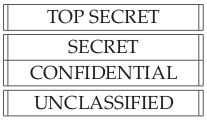
\includegraphics[scale=0.6]{pics/multilevelSecurity.png}
			\end{figure}

			The access control policy was simple: an official could read a document
			only if his {\bf clearance} was at least as high as the document’s classification. 
			So an official cleared to ‘Top Secret’ could read a ‘Secret’ document, but not vice
			versa. The effect is that information may only flow upwards, from confidential
			to secret to top secret, but it may never flow downwards unless an authorized
			person takes a deliberate decision to declassify it.

		\subsection{Information Flow Control}
			It was in this context of the classification of government data that the 
			{\bf Bell- LaPadula or BLP model} of computer security was formulated in 1973. 
			It is also known as multilevel security and systems which implement it are often
			called {\bf multilevel secure or MLS systems}. 
			Their basic property is that information cannot flow downwards.
			More formally, the Bell-LaPadula model enforces two properties:

				\begin{itemize}
					\item {\bf The simple security property:} no process may read data 
					at a higher level. This is also known as no read up (NRU);
					\item {\bf The *-property:} no process may write data to a lower level. 
					This is also known as no write down (NWD).
				\end{itemize}

			So we must prevent programs running at ‘Secret’ from writing to files at
			‘Unclassified’, or more generally prevent any process at High from signalling
			to any object (or subject) at Low. In general, when systems enforce a security
			policy independently of user actions, they are described as having 
			{\bf mandatory access control}, as opposed to the {\bf discretionary access control} 
			in systems like Unix where users can take their own access decisions about their files.


		\subsection{Criticisms of Bell-LaPadula}
			The introduction of BLP caused a lot of excitement: here was a straightforward
			security policy which was clear to the intuitive understanding yet still allowed
			people to prove theorems. But John McLean showed that the BLP rules
			were not in themselves enough. 
			He introduced System Z, defined as a BLP system with the added feature that a 
			user can ask the system administrator to temporarily declassify any file from 
			High to Low. In this way, Low users can read any High file without breaking the 
			BLP assumptions.
			
			Bell’s argument was that {\bf System Z cheats} by doing something the model
			doesn’t allow (changing labels isn’t a valid operation on the state), and
			McLean’s argument was that it didn’t explicitly tell him so. The issue is dealt
			with by introducing a tranquility property. 

			{\bf The strong tranquility property} says that security labels never change 
			during system operation.\\
			{\bf The weak tranquility property} says that labels never change in such a way 
			as to violate a defined security policy.

			The motivation for the weak property is that in a real system we often
			want to observe the principle of least privilege and start off a process at the
			uncleared level, even if the owner of the process were cleared to ‘Top Secret’.
			If she then accesses a confidential email, her session is automatically upgraded
			to ‘Confidential’; and in general, her process is upgraded each time it accesses
			data at a higher level. {\bf This is known as the high water mark principle}. 
			As subjects are usually an abstraction of the memory management sub-system
			and file handles, rather than processes, this means that state changes when
			access rights change, rather than when data actually moves.

			Finally it’s worth noting that even with the high-water-mark refinement,
			BLP still doesn’t deal with the creation or destruction of subjects or objects
			(which is one of the hard problems of building a real MLS system).

			\clearpage
			\subsection{Alternative Formulations}

				The first multilevel security policy was a version of high water mark.
				There is a lot of other formulations of multilevel security.

				\begin{itemize}
					\item {\bf Noninterference} was introduced by Joseph Goguen and Jose Meseguer 
					in 1982. In a system with this property, High’s actions have no effect on
					what Low can see. The motive for nondeducibility is to find a model that can deal with applications such as a LAN on which there are machines at both Low 
					and High, with the High machines encrypting their LAN traffic.
					\item {\bf Generalized Noninterference and restrictiveness}. The
					former is the requirement that if one alters a high level input event in a 
					legal sequence of system events, the resulting sequence can be made legal by, 
					at most, altering one or more subsequent high-level output events. The latter
					adds a further restriction on the part of the trace where the alteration of 
					the high-level outputs can take place. This is needed for technical reasons 
					to ensure that two systems satisfying the restrictiveness property can be composed into a third which also does. 
					\item {\bf The Harrison-Ruzzo-Ullman model} tackles the problem of how to 
					deal with the creation and deletion of files, an issue on which BLP is silent. 
					\item {\bf Compartmented Mode Workstation (CMW)} policy,
					which attempted to model the classification of information using floating
					labels, as opposed to the fixed labels associated with BLP.
					\item {\bf The type enforcement model} assigns subjects to domains and 
					objects to types, with matrices defining permitted domain-domain and 
					domain-type interactions.
					\item {\bf Role-based access control (RBAC)}. This provides a more general
					framework for mandatory access control than BLP in which access decisions 
					don’t depend on users’ names but on the functions which they are currently
					performing within the organization. 
				\end{itemize}

			\clearpage
			\subsection{The Biba Model}
				Many refer the Biba Model as the {\bf ‘Bell-LaPadula upside down’}. 
				The Biba model deals with integrity alone and ignores confidentiality. 
				The key observation is that confidentiality and integrity are in some sense 
				dual concepts:\\
				{\bf Confidentiality} is a constraint on who can read a message, while \\
				{\bf Integrity} is a constraint on who can write or alter it.

				To model such a system, we can use a multilevel integrity policy with the
				rules that we {\bf can read data at higher levels and write to lower levels}, 
				but we must {\bf never read down or write up}, as either could allow High 
				integrity objects to become contaminated with Low — that is potentially 
				unreliable — data. 
				The Biba model is often formulated in terms of the {\bf low water mark principle},
				which is the dual of the high water mark principle discussed above: 
				the integrity of an object is the lowest level of all the objects that contributed
				to its creation.

				Vista marks file objects with an integrity level, which can be Low, Medium,
				High or System, and implements a default policy of NoWriteUp. Critical Vista
				files are at System and other objects are at Medium by default — except for
				Internet Explorer which is at Low. The effect is that things downloaded using
				IE can read most files in a Vista system, but cannot write them. The idea is to
				limit the damage that can be done by viruses and other malware. 














